%%%%%%%%%%%%%%%%%%%%%%%%%%%%%%%%%%%%%%%%%%%%%%%%%%%%%%%%%%%%%%%%%%%%%%%%%%%%%%%
%                         File: osa-revtex4-1.tex                             %
%                        Date: April 15, 2013                                 %
%                                                                             %
%                              BETA VERSION!                                  %
%                   JOSA A, JOSA B, Applied Optics, Optics Letters            %
%                                                                             %
%            This file requires the substyle file osajnl4-1.rtx,              %
%                   running under REVTeX 4.1 and LaTeX 2e                     %
%                                                                             %
%                   USE THE FOLLOWING REVTeX 4-1 OPTIONS:                     %
% \documentclass[osajnl,twocolumn,showpacs,superscriptaddress,10pt]{revtex4-1}%
%                    %% Use 11pt for Applied Optics                           %
%                                                                             %
%               (c) 2013 The Optical Society of America                       %
%                                                                             %
%%%%%%%%%%%%%%%%%%%%%%%%%%%%%%%%%%%%%%%%%%%%%%%%%%%%%%%%%%%%%%%%%%%%%%%%%%%%%%%

\documentclass[osajnl,twocolumn,showpacs,superscriptaddress,10pt]{revtex4-1} %% use 11pt for Applied Optics
%\documentclass[osajnl,preprint,showpacs,superscriptaddress,11pt]{revtex4-1} %% use 12pt for preprint option
\usepackage{amsmath,nccmath,amssymb,graphicx,float,minted,xparse,tikz}
\usepackage[utf8]{inputenc}
\graphicspath{{images/}}

\usepackage{mathtools,enumitem}
\usepackage{minted}

\begin{document}

\title{Programación Distribuida y Tiempo Real}

\author{Ulises Jeremias Cornejo Fandos}
\affiliation{Licenciatura en Informática, Facultad de Informática, UNLP}

\maketitle %% required

\section{Utilizando como base el programa ejemplo de RMI:}

\subsection{Analice si RMI es de acceso completamente transparente (access transparency, tal como 
está definido en Coulouris-Dollimore-Kindberg). Justifique.}

\textit{Ver definición de transparency según Coulouris-Dollimore-Kindberg en la sección \ref{apendix:1a}} \\

Dada la sintaxis y nomenclatura de las operaciones definidas, no es sensillo definir si las mismas
serán operaciones locales o remotas. Sin embargo, se debe realizar un lookup del nombre de las clases
en momento de invocacion de las mismas teniendo en cuenta el host remoto, pues no están en el
espacio de nombres local.

Esto nos indica que, si bien a nivel de métodos no tenemos forma a priori de determinar si una
operación es local o remota, pues no hay real diferencia en la invocación de una u otra,
si la hay al momento de obtener la clase remota.

Además, se tiene en cuenta el manejo de errores dados en la comunicación dado que el método
remoto tiene a fallar con mayor frecuencia que el método local por fallas en la comunicación. \\

Por lo tanto, RMI ofrece transparencia de acceso al permitir invocar de la misma forma un procedimiento
local y uno remoto. Sin embargo, la transparencia es parcial dado que se tienen en cuenta
otras cuestiones como el lookup de las clases remotas y errores en la comunicación.

\subsection{Enumere los archivos .class que deberían estar del lado del cliente y del lado del servidor y
que contiene cada uno.}

\textit{A continuación se enumeran los archivos .class con información de cada uno de ellos:}

\begin{itemize}
    \item \textbf{AskRemote.class}
    
    Este archivo presente en el cliente identifica a la clase Cliente 
    que realiza el llamado al método remoto. Contiene información de conexión al servidor (\textit{hostname}, \ldots),
    invocacion a la clase y método remoto.

    \item \textbf{StartRemoteObject.class}
    
    En este archivo dispuesto en el servidor se define la clase encargada de instanciar a la clase contenedora de los métodos remotos a invocar y la registra
    en el espacio de nombres asegurándose que pueda ser llamada por el cliente.

    \item \textbf{IfaceRemoteClass.class}
    
    Este archivo se dispone del lado del servidor y contiene la declaración de la interface en la cual
    se definen los métodos que el servidor debe implementar para que puedan ser invocados.

    \item \textbf{RemoteClass.class}
    
    En este archivo dispuesto del lado del servidor se encuentra la implementación de los métodos definidos en la
    interface anteriormente mencionada, \textit{IfaceRemoteClass}, para que puedan
    ser invocados remotamente. Extiende de \textit{UnicastRemoteObject} que hace que toda la comunicación
    sea completamente transparente al programador de este lado.
\end{itemize}

\section{Identifique similitudes y diferencias entre RPC y RMI.}

La principal diferencia entre RPC y RMI radica en el paradigma, y esto
se debe a que RMI involucra objetos.
En lugar de llamar procedimientos de forma remota, se llaman a métodos de
objetos remotos. \textit{Se podría afirmar que RMI es la version orientada a objetos
de RPC.} En RMI cada objeto tiene una referencia única en todo el sistema,
tanto si los objetos son remotos como locales, permitiendo así el pasó de
objetos como parámetros, herencia y relaciones entre objetos remotos,
ofreciendo un pasaje de parámetros con una mayor riqueza semántica y un
mayor nivel de abstracción que en RPC, donde solo se pueden pasar
parámetros por valor.

Sin embargo, en ambos modelos los detalles de implementación están ocultos al usuario
y los métodos o procesos disponibles se conocen a través de una interfaz
que provee el servidor.

Ambos ofrecen un alto nivel de transparencia de acceso, donde los llamadas remotas
y locales poseen la misma sintáxis, pero las interfaces remotas
diferencian la naturaleza distribuida de las llamadas remotas al, por
ejemplo, soportar excepciones remotas o tener en cuenta posibles fallas
en la comunicación con tiempos de timeout.

\section{Investigue porque con RMI puede generarse el problema de desconocimiento de clases en
las JVM e investigue como se resuelve este problema.}

En RMI puede ser que los métodos de un objeto remoto admitan como parámetros a otras clases y devuelvan clases.  Por lo que un metodo remoto podría devolver un objeto o admitir un parámetro de una clase desconocida para el cliente. En ese caso se podría generar una ClassNotFoundException
Por ejemplo, puede ser un método así

\begin{minted}{java}
public IResult get(IParam arg)
throws java.rmi.RemoteException
{
    ...
}
\end{minted}


Una solucion sería que  tanto el servidor como el cliente tengan sus propias copias de las clases que implementen estas interfaces. Es decir, si ClaseResultado implementa InterfaceResultado y ClaseParametro implementa InterfaceParametro, tanto el cliente como el servidor deben tener en su CLASSPATH los ficheros ClaseResultado.class y ClaseParametro.class. Esto no sería una solucion deseada, ya que se deben saber todas las clases que utiliza el servidor y copiarlas del lado del cliente, quitando dinamismo y escalabilidad a rmi.
La solución provista por RMI es instalar \textit{RMISecurityManager}, el cual habilita la carga dinámica de clases. De esta forma el servidor no necesita tener una copia de ClaseParametro.class ni el cliente una copia de ClaseResultado.class. 

\section{Implementar con RMI el mismo sistema de archivos remoto implementado con RPC en la
práctica anterior:}

Para esto se utilizó la estructura de archivos del ejemplo. Se definió
una interfaz con 3 métodos, \textit{read}, \textit{write} y
\textit{list} \\

Tanto el cliente como el servidor, se alimentan de la interfaz definida
en IfaceFTServer donde la clase que los implementa es la clase FTServer.

Luego, se implementa un cliente que interactúe contra el servidor, con
los comandos basicos, nombrados anteriormente. Esto se hizo en la clase
FTClient. El servidor, utiliza la implementación de la clase FTServer, y
corre instanciando un objeto de la clase StartRemoteObject.

\section{Investigue si es posible que varias invocaciones remotas estén ejecutándose
concurrentemente y si esto es apropiado o no para el servidor de archivos del ejercicio
anterior. En caso de que no sea apropiado, analice si es posible proveer una solución
(enunciar/describir una solución, no es necesario implementarla). Nota: diseñe un
experimento con el que se pueda demostrar fehacientemente que dos o más invocaciones
remotas se ejecutan concurrentemente o no. Compare este comportamiento con lo que
sucede con RPC.}

Al funcionar sobre Java, RMI admite concurrencia nativa. Sin embargo,
el principal inconveniente en RMI, es que no maneja multihilos de manera
segura, es decir, los llamados pueden causar colisiones en los recursos
del servidor. 
Para evitar esto, se pueden utilizar mecanismos conocidos para sincronización,
aunque RMI no provee ninguno por su cuenta. \\

En la presente implementación, se cuenta con 2 comandos seguros para la concurrencia,
\textit{read} y \textit{list}, y el comando \textit{write} el cual no lo es. \\

El principal inconveniente que puede traer la ejecución de comandos no seguros, es
la perdida de datos en el servidor.

Para demostrar la concurrencia de RMI, se utilizó un comando extra, para
mayor simplicidad del experimento. En este caso, el método remoto solamente
genera un sleep de 6 minutos. El experimento puede ser la ejecución de este comando por dos clientes
interactuando con el mismo servidor.

\begin{figure}[H]
    \centering
    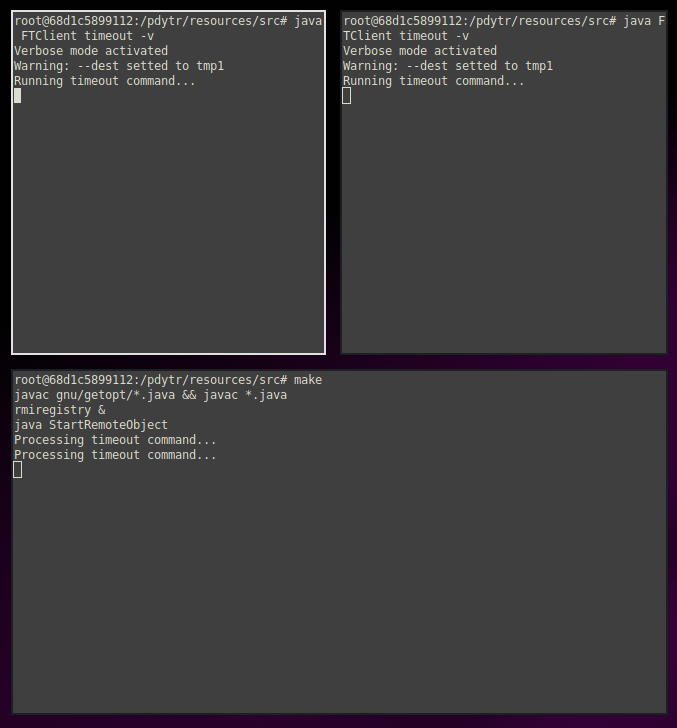
\includegraphics[width=0.45\textwidth]{concu}
    \caption{Experimento de concurrencia en servidor}.
    \label{figure:concu}
\end{figure}

\section{Tiempos de respuesta de una invocación:}

\subsection{Diseñe un experimento que muestre el tiempo de respuesta mínimo de una invocación con
JAVA RMI. Muestre promedio y desviación estándar de tiempo respuesta.}

Se realizan 10 experimentos en los cuales se ejecuta el comando \textit{time} del cliente y se almacenan
los tiempos, en milisegundos, impresos en un archivo. Para esto se utiliza la misma instancia del proceso servidor. \\

Se puede volver a generar el archivo corriendo el script \textit{./bin/run --build [-s X] [-p Y] [-o PATH]}
el cual acepta como parametro $X$ la cantidad de iteraciones, como parametro $Y$ la cantidad de reintentos en caso de error de conexión y como parámetro \textit{PATH} el nombre de archivo donde dejar los valores.

La desviación estandar obtenida es 17579823 y la media es 657661.

\subsection{Investigue los timeouts relacionados con RMI. Como mínimo, verifique si existe un timeout
predefinido. Si existe, indique de cuanto es el tiempo y si podría cambiarlo. Si no existe,
proponga alguna forma de evitar que el cliente quede esperando indefinidamente.}

El paquete \textbf{java.rmi} no cuenta con timeout configurable,
se puede utilizar el paquete \textbf{sun.rmi}, el cual cuenta con una
propiedad configurable de timeout.

De no utilizarse \textbf{sun.rmi}, se pueden llegar a trabajar con algun
timer o algo similar, pero no hay ninguna herramienta que nos brinde 
\textbf{java.rmi} para dicho fin.

\section{Apéndice}

\subsection{Coulouris-Dollimore-Kindberg}
\label{apendix:1a}

Access transparency. Enables local and remote resources to be
accessed using identical operations They both offer a similar level
of transparency that is, local and remote calls employ the same
syntax but remote interfaces typically expose the distributed nature
of the underlying call, for example by supporting remote exceptions

\end{document}
